% !TEX program = latexmk
%%%%%%%%%%%%%%%%%%%%%%%%%%%%%%%%%%%%%%%%%%%%%%%%%%%%%%%%%%%%%%%%%%%%%%%%%%%%%%%%%%%%%%%%%%%%%%
% Template Beamer Sugestivo para Projetos EMAp
% by Renato Rocha Souza / Eduardo Mendes
% Based on MIT Beamer Template
%%%%%%%%%%%%%%%%%%%%%%%%%%%%%%%%%%%%%%%%%%%%%%%%%%%%%%%%%%%%%%%%%%%%%%%%%%%%%%%%%%%%%%%%%%%%%% 

%\documentclass{beamer} %voce pode usar este modelo tambem
\documentclass[handout,t,usenames,dvipsnames]{beamer}
\usepackage{graphicx,url}
\usepackage[brazil, english]{babel}   
\usepackage[utf8]{inputenc}
\usepackage{booktabs}
\usepackage{setspace}
\usepackage{ragged2e}
\usepackage{tabularx}
\usepackage{multirow,array}
\usepackage{arydshln}
\usepackage{natbib}

\graphicspath{}
\batchmode
\usepackage{pgfpages}
\pgfpagesuselayout{4 on 1}[a4paper,landscape,border shrink=5mm]
\usepackage{amsmath,amssymb,enumerate,epsfig,bbm,calc,color,ifthen,capt-of}
%\usetheme{Warsaw}
\usecolortheme{emap}



\defbeamertemplate{footline}{page number}{%
\vskip1pt%
\setbeamertemplate{footline}[page number]%
\usebeamertemplate{footline}%
}
\setbeamertemplate{footline}[page number]


%-------------------------Titulo/Autores/Orientador------------------------------------------------
\date{}
\title{\large{Learning about Corruption:} \\ 
\vspace{1em}
\large{A Statistical Framework for working with Audit Reports}}
\date{}
\author{by Laura Sant'Anna and Duda F. Mendes} 

%-------------------------Logo na parte de baixo do slide------------------------------------------
%\pgfdeclareimage[height=1.2cm]{emap-logo}{Logo_FGV_EMAp.png}
%\logo{\pgfuseimage{emap-logo}\hspace*{0.1cm}}

%-------------------------Este código faz o menuzinho bacana na parte superior do slide------------
\AtBeginSection[]
{
\begin{frame}<beamer>
\frametitle{Outline}
\tableofcontents[currentsection]
\end{frame}
}
\beamerdefaultoverlayspecification{<+->}
% -----------------------------------------------------------------------------
\begin{document}
% -----------------------------------------------------------------------------

%---Gerador de Sumário---------------------------------------------------------
\frame{\titlepage}
\section[]{}
\begin{frame}{Content}
\tableofcontents
\end{frame}
%---Fim do Sumário------------------------------------------------------------


%--------------------------------------------------------------------------------


\section{Motivation}


\begin{frame}{Motivation}
%\justifying
\vspace{1em}
\onehalfspacing

Quantitative studies in corruption are essential to track externalities and to guide effective public policies to fight against it.
\vspace{1em}

But corrupt acts are hard to be traced and accounted for, therefore data about it is scarce.

\vspace{1em}
\begin{itemize}
%\justifying
\item Cross-country indicators of corruption are usually based on perception, such as the \textit{CPI} from Transparency International and the \textit{CPIA transparency, accountability, and corruption in the public sector rating} from World Bank.
\end{itemize}

\end{frame}

\begin{frame}{Motivation}

\justifying
\vspace{1em}

In Brazil, CGU was created in 2003 to assist in activities of internal control, such as public auditing and fighting against corruption.
\vspace{2em}

The CGU Random Audits Anti-Corruption Program (\textit{Programa de Fiscalização por Sorteios Públicos}) has contributed to overcome data scarcity and has been widely used by researchers in Economics and Political Sciences.
\vspace{1em}

\begin{itemize}
    \item Nevertheless, the use of reports from this program is sub-optimal: most researchers read and manually classify just a small sample to construct corruption indicators.
\end{itemize}

\end{frame}

\begin{frame}{Motivation}
\onehalfspacing
%\justifying
\vspace{1em}
\small
\textcolor{emap-azul-escuro}{Ferraz and Finan (2008)\nocite{Eleicoes}}: found evidence that public disclosure of audit reports before local elections contributed to reduce in 17\% the expected probability of reelection of mayors in municipalities where corruption was detected.
\vspace{2em}


\textcolor{emap-azul-escuro}{Ferraz, Finan and Moreira (2012)\nocite{Educacao}}: found evidence that schooling outcomes are significantly worse in municipalities where corruption in education was detected.
\vspace{2em}

\textcolor{emap-azul-escuro}{Lichand, Lopes and Medeiros (2016)\nocite{Saude}}: found evidence that, although the program contributed to reduce irregularities associated to corruption, it was not followed by an improvement in municipal health basic services.

\end{frame}

\begin{frame}{Motivation}
\vspace{0.8em}
{\color{emap-azul-escuro}\Large Research goals}
\doublespacing
\begin{enumerate}
%\justifying
\item To propose a framework for working with text data in inferential models, using irregularities detected during the CGU anti-corruption program audits as a particular case.
\vspace{1em}
\item To construct and publicly release a dataset of irregularities categorized through a supervised learning task.
\end{enumerate}
\end{frame}


%--------------------------------------------------------------------------------


\section{CGU Random Audits Anti-Corruption Program}

\begin{frame}{CGU Random Audits Anti-Corruption Program}
\vspace{1em}

\begin{itemize}
%\justifying
\item Randomly selects small and medium municipalities for auditing of federal transfers.
\vspace{1em}

\item Inspects federal transfers associated to ministries of Education, Health, Social Development, National Integration, Cities, Agricultural Development and others, depending on the edition.
\vspace{1em}

\item Available in pdf: 2,241 reports of audits conducted between 2003-2015  (40 editions).
\vspace{1em}

\item Dataset of irregularities (obtained through \textit{LAI}): 81,715 irregularities detected in the 1,223 audits conducted between 2006-2015 (20 editions).
\end{itemize}

\end{frame}

\begin{frame}{CGU Random Audits Anti-Corruption Program}
\begin{figure}[h!]
%\label{fig:distClass}
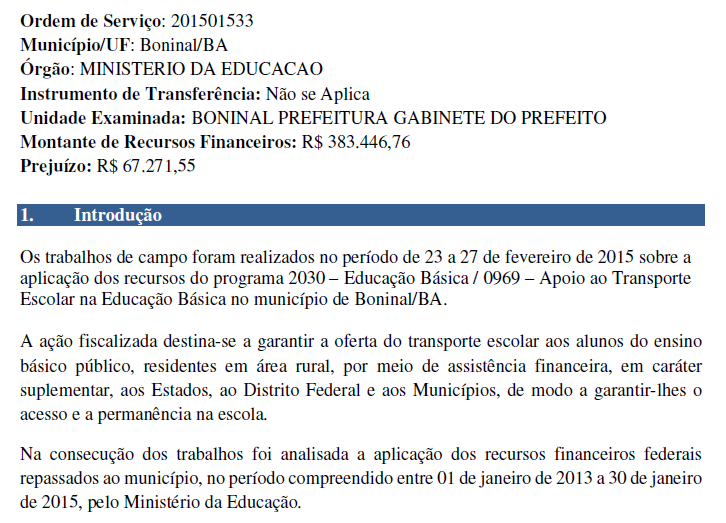
\includegraphics[width=8cm]{ex_OS.png}
\centering
\caption{\small Example of Service Order in Education executed in Boninal (BA)}
\end{figure}
\end{frame}

\begin{frame}{CGU Random Audits Anti-Corruption Program}
\vspace{1em}
\small
\textit{Severe} irregularities:
\begin{itemize}
\justifying
    \item[--]``Exigências indevidas com repercussão na competitividade do certame e direcionamento em licitação do transporte escolar (Pregão n.º 012/2013)''
    \item[--]``Falta de comprovação documental das despesas realizadas em 2013 e 2014.''
    \item[--]``Pagamento por serviços não realizados, no montante de R\$13.577,27, referente à despesa do transporte escolar do mês de junho de 2013.''
    \item[--]``Intermediação irregular na prestação do serviço de transporte escolar.''
\end{itemize}
\textit{Moderate} irregularity:
\begin{itemize}
    \item[--]``O Conselho do Fundeb não atua no acompanhamento da execução do Programa Nacional de Transporte Escolar - Pnate.''
\end{itemize}
\end{frame}

\begin{frame}{CGU Random Audits Anti-Corruption Program}
\vspace{1em}
\onehalfspacing
\justifying

And its conclusion was:
\vspace{1em}

``Com base nos exames realizados, conclui-se que a aplicação dos recursos federais recebidos está inadequada aos normativos referentes ao objeto fiscalizado. A Prefeitura de Boninal/BA contratou e pagou irregularmente uma cooperativa para a prestação do serviço de transporte escolar. O desvio de recursos, apesar de efetivo, é de difícil mensuração com as informações disponibilizadas à Fiscalização.''
\end{frame}


%--------------------------------------------------------------------------------


\section{Methodology}


\begin{frame}{Methodology}
\vspace{0.8em}

{\color{emap-azul-escuro}Automate Text Classification}
\begin{enumerate}
\item Manual classification of irregularities
\item Supervised learning for classification of irregularities
\end{enumerate}

\vspace{0.8em}
{\color{emap-azul-escuro}Model estimation with Measurement Error}\\
\begin{enumerate}
\item Construction of a municipal indicator of corruption
\item Model estimation adjusting for measurement error
\end{enumerate}

\vspace{2em}
{\color{emap-azul-escuro}\large Case Study}: Does corruption in educational funds affect schooling outcomes?


\end{frame}


%--------------------------------------------------------------------------------


\section{Results}

\begin{frame}{Automate Text Classification}
\justifying
{\color{emap-azul-escuro}\large Manual classification of irregularities}
\vspace{0.5em}
\small

We randomly selected 4,200 irregularities (5\% of the sample) to classify into 12 well-delimited classes, based on Ferraz and Finan (2008)\nocite{Eleicoes} and Lichand, Lopes and Medeiros (2012)\nocite{Saude}:
\begin{table}
\footnotesize
\centering
    \begin{tabular}{ | p{5cm}| p{5cm} |}
    \hline
    Associated to public corruption & Other \\ \hline
     {} & \scriptsize{Councils and public secretaries (IM)}\\
     Procurement related flaws (FL) & \scriptsize{Mismanagement practices in the municipal government (MM)}\\
     Over-invoicing (SF) & \scriptsize{Poorly evaluated public services and facilities (IF)}\\
     Resource Diversion (DR) & \scriptsize{Unfinished projects and goals in public construction (OB)}\\ 
     {} & \scriptsize{Frauds in public programs (FD)}\\
     {} & \scriptsize{Human resources anomalies (RH)}\\
     {} & \scriptsize{Incomplete documentation (DOC)}\\
     {} & \scriptsize{Lack or divergence on published information (INFO)}\\
     {} & \scriptsize{Absence of State's government participation (RE)}\\ \hline
    \end{tabular}
\end{table}


\vspace{1em}
 
\end{frame}

\begin{frame}{Automate Text Classification}
\justifying
\small
Related to public corruption:

\begin{itemize}
\justifying
    \item[--] {\color{emap-azul-escuro}[FL]} ``Exigências indevidas com repercussão na competitividade do certame e direcionamento em licitação do transporte escolar (Pregão n.º 012/2013)''
    \item[--] {\color{emap-azul-escuro}[DR]} ``Falta de comprovação documental das despesas realizadas em 2013 e 2014.''
    \item[--] {\color{emap-azul-escuro}[DR]} ``Pagamento por serviços não realizados, no montante de R\$13.577,27, referente à despesa do transporte escolar do mês de junho de 2013.''
\end{itemize}
\vspace{0.5em}

Not related to public corruption: 
\begin{itemize}
\justifying
    \item[--] {\color{emap-azul-escuro}[IF]}``Intermediação irregular na prestação do serviço de transporte escolar.''
    \item[--] {\color{emap-azul-escuro}[IM]}``O Conselho do Fundeb não atua no acompanhamento da execução do Programa Nacional de Transporte Escolar - Pnate.''


\end{itemize}

\end{frame}

\begin{frame}{Automate Text Classification}
\justifying
{\color{emap-azul-escuro}\large Manual classification of irregularities}
\vspace{0.5em}

\begin{figure}[h!]
%\label{fig:distClass}
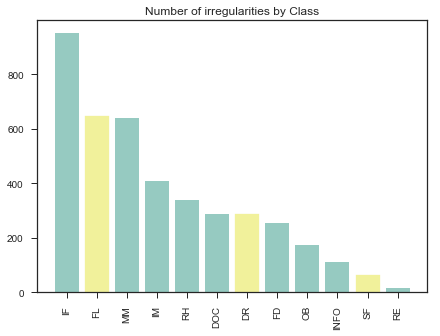
\includegraphics[width=7cm]{irreg_class.png}
\centering
\caption{Number of irregularities manually assigned to each class}
\end{figure}
 
\end{frame}

\begin{frame}{Automate Text Classification}
\begin{table}[h]
\tiny
\begin{center}
    \centering
\label{table:freqWords}   
 \begin{tabular}{p{1.5cm} p{2cm} p{2cm} p{2cm}} 
 \toprule
 \textbf{Class} & \multicolumn{3}{c}{\textbf{frequent tokens} (relative frequency)}\\\midrule
 FL & licitatório (0.35) & processo (0.3) & licitação (0.23) \\ \midrule
 SF & valor (0.35)  & sobrepreço (0.32) & preço (0.31) \\ \midrule
 DR & \textcolor{Maroon}{recurso} (0.47) & \textcolor{Maroon}{despesa} (0.45) & pagamento (0.29) \\ \midrule
 FD &  \textcolor{Maroon}{programa} (0.62) & beneficiário (0.56) & família (0.53) \\ \midrule
 IM & conselho (0.49) & municip (0.38) & social (0.24) \\ \midrule
 MM &  \textcolor{Maroon}{recurso} (0.42) &  \textcolor{Maroon}{ausência} (0.26) & notificação (0.15) \\ \midrule
 IF & control (0.16) & escolar (0.14) &  \textcolor{Maroon}{programa} (0.12) \\ \midrule
 OB & obra (0.63) & execução (0.32) & objeto (0.16) \\ \midrule
 RH & saúd (0.32) & profissional (0.25) & equip (0.21) \\ \midrule
 DOC &  \textcolor{Maroon}{ausência} (0.28) & \textcolor{Maroon}{despesa} (0.25) & documento (0.24) \\ \midrule
 INFO & divergência (0.33) & censo (0.27) & beneficiário (0.25) \\ \midrule
 RE & contrapartida (0.81) & estadu (0.56) &  \textcolor{Maroon}{ausência} (0.5) \\ \midrule
\end{tabular}
\end{center}
\caption{Three most frequent (stemmized) tokens in each class and share of irregularities that contain it}
\end{table}
 
\end{frame}

\begin{frame}{Automate Text Classification}
\justifying
{\color{emap-azul-escuro}\large Supervised Learning for Text Classification}
\vspace{0.5em}

Considering five classifiers - Naive Bayes, Multinomial Logistic Regression, SVM, Random Forest and a Voting ensemble method - we perform the following steps:
\vspace{0.5em}

\small
\begin{enumerate}
\justifying
    \item Text mining: text pre-processing, exploratory analysis, feature generation
    \item 10-fold cross-validation for choosing each algorithm's hyper-parameters (eg. number of text features, regularization term, n-gram range). Evaluate model performance when non-textual features are also included.
    \item Train each classifier using the hyper-parameters that minimize the cross-validation error.
    \item 10-fold cross-validation to compute accuracy, precision and recall for each model and choose one as our final classifier.
\end{enumerate}
 
\end{frame}

\begin{frame}{Automate Text Classification}


\begin{figure}[h!]
%\label{fig:distClass}
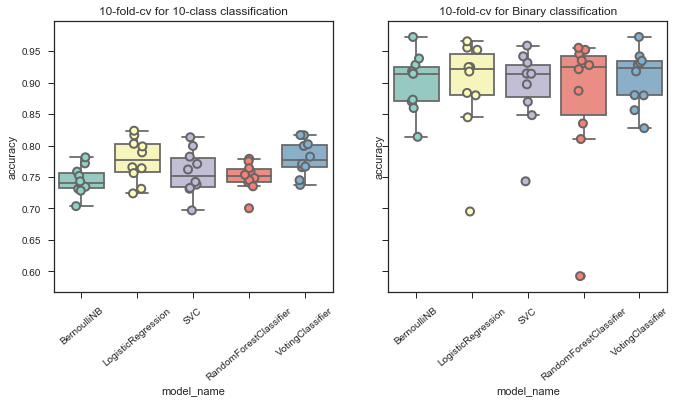
\includegraphics[width=9cm]{cv.png}
\centering
\caption{10-fold cross-validation for Supervised Learning tasks}
\end{figure}
 
\end{frame}

\begin{frame}{Automate Text Classification}


\begin{columns}
\begin{column}{0.5\textwidth}
    \begin{center}
     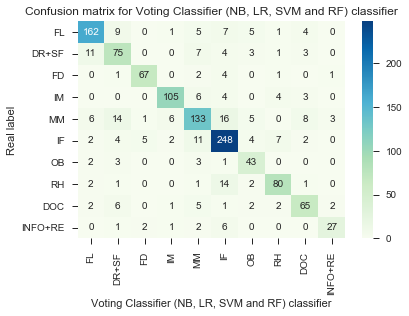
\includegraphics[width=1\textwidth]{matrix_10.png}
     \end{center}
\end{column}
\begin{column}{0.5\textwidth}  %%<--- here
    \begin{center}
     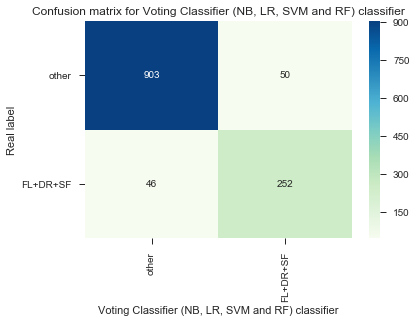
\includegraphics[width=1\textwidth]{matrix_2.png}
     \end{center}
\end{column}
\end{columns}

\centering
{\color{emap-azul-escuro}\small Figure:} \small Confusion matrices on the test set using Voting classifier
\end{frame}

%PENSAR O QUE FAZER COM ESSE SLIDE
\begin{frame}{Automate Text Classification}

{\color{emap-azul-escuro}\large Supervised Learning for Text Classification}
\vspace{0.5em}
\justifying

\small
For the Model estimation step, it is convenient to write the joint probabilities taken from the normalized confusion matrix as:

\vspace{1em}
  \begin{table}[h!]
  \label{eq:conf_matrix}
    \setlength{\extrarowheight}{2pt}
    \centering
    \begin{tabular}{c c|p{1cm}|p{1cm}|}
      & \multicolumn{1}{c}{} & \multicolumn{2}{c}{Predicted label}\\
      & \multicolumn{1}{c}{} & \multicolumn{1}{c}{0}  & \multicolumn{1}{c}{1} \\\cline{3-4}
      \multirow{2}*{True label}  & 0 & $\pi_{00}$  & $\pi_{01}$ \\\cline{3-4}
      & 1 & $\pi_{10}$ & $\pi_{11}$\\\cline{3-4}
    \end{tabular}
  \end{table}
\end{frame}

\begin{frame}{Model estimation with Measurement Error}
\justifying
{\color{emap-azul-escuro}\large Constructing a Municipal Indicator of Corruption}
\vspace{0.5em}
\small

For each municipality $i$ we have $N_i$ irregularities $D_j$ classified as 1 (associated to corrupt practices) or 0. An indicator variable of corruption for municipality $i$ is:
  \begin{align*}
    C_i=
    \begin{cases}
      1, & \text{if}\ \exists D_{i,j}=1 \\
      0, & \text{otherwise}.
    \end{cases}
  \end{align*}
Since we want an indicator of corruption in Education, we observe three conditions:
\begin{enumerate}
    \item \small It is associated to a OS expedited by the Ministry of Education,
    \item \small It is predicted as FL, SF or DR on the automated classification task,
    \item \small It is classified as \textit{Severe} by CGU.
\end{enumerate}
According to this criteria, in approximately 41\% of the audits, at least one irregularity associated to corruption in education was detected.
\end{frame}

\begin{frame}{Model estimation with Measurement Error}
\justifying
\small
We want to use this indicator as explanatory variable in a regression model. Note that it was constructed with a measurement error:
$$ C = Z + U_{C}$$
Thus, given $X = [Z\ \ : \ \ W]$ we have the following model:
\begin{align*}
    \begin{split}
        Y &= X \beta + E\\
        &= (X_{M} - U) \beta + E\\
        &= X_{M}\beta + E - U\beta.
        \end{split}
\end{align*}
We can show that the OLS estimate in this case is asymptotically biased and, using extra-sample information, we can take an MLS approach Johnson (1997) and Savoca (2000)\nocite{book:johnston, Savoca} to correct for measurement error:
\begin{align*}
    \hat{\beta}_{MLS} = (I - \hat{\Omega})^{-1} \hat{\beta}_{OLS},
\end{align*}
where $\hat{\Omega}$ is an estimator for $\Omega = \Sigma^{-1}_{X_{M}} \Sigma_{X_{M},U}$. 
\end{frame}

\begin{frame}{Model estimation with Measurement Error}
\justifying
\small
\vspace{1em}
\[
   \hat{\beta}_{MLS} = \left[
\begin{array}{c}
\hat{\alpha}_{MLS}  \\
\hdashline[2pt/2pt]
\hat{\theta}_{MLS}
\end{array}
\right],    \quad \hat{\beta}_{OLS} = \left[
\begin{array}{c}
\hat{\alpha}_{OLS}  \\
\hdashline[2pt/2pt]
\hat{\theta}_{OLS}
\end{array}
\right],
\]
\[
\Sigma_{X_{M}}^{-1}=
\left[
\begin{array}{c;{2pt/2pt}c}
\sigma^2_{C} & \sigma_{C,W} \\
\hdashline[2pt/2pt]
\sigma_{W,C} & \Sigma_{W}
\end{array}
\right]^{-1}, \quad  \Sigma_{X_{M}U}= \left[
\begin{array}{c;{2pt/2pt}c}
\sigma_{C,U_C} & \sigma_{C,0} \\
\hdashline[2pt/2pt]
\sigma_{W,U_C} & \Sigma_{W,0}
\end{array}
\right].
\]
Assuming that variables in $W$ have no measurement error: $\sigma_{C,0}=0$ and $\sigma_{W,0}=0$. Since the error $U_C$ is a consequence of the text classification, it is not correlated with municipal variables in $W$: $\sigma_{W,U_C}=0$. Thus:
\begin{align*}
\label{MLS_true}
    \begin{split}
    \hat{\alpha}_{MLS} = \Big(1 - \frac{\sigma_{Z,U_c} \sigma^2_{U_c}}{\sigma^2_{C} - \sigma_{C,W}\Sigma_W^{-1}\sigma_{W,C}} \Big) ^{-1} \cdot \hat{\alpha}_{OLS},
    \end{split}
\end{align*}
\small where $\sigma_{Z,U_c}$ and $\sigma^2_{U_c}$ can be estimated with a closed-form using $P, r_{01}, r_{10}$ and the denominator term can be estimated using the inverse of the sample covariance matrix.

\end{frame}

\begin{frame}{Model estimation with Measurement Error}
\justifying
\vspace{0.5em}

Besides constructing a municipal indicator, we need an estimate for its measurement error. 
\vspace{0.5em}

Particularly, the conditional probability of municipality $i$ being misclassified as ``corrupt'' when it is not (\textit{false positive} rate), can be calculated through:
\begin{align*}
    r_{10,i} = \mathbb{P}(\hat{C_i}=1|C_i=0, N_i) &= \mathbb{P}(\exists \{\hat{D_{ij}} = 1\} | \nexists \{D_{ij} = 1\})
\end{align*}

The case is analogous for the \textit{false negative} rate and taking the expected values on $N_i$, we have:
\begin{align*}
    \begin{split}
    r_{10} = 1 - \mathbb{E}\Big[\Big(\frac{\pi_{00}}{\pi_{00}+\pi_{10}}\Big)^{N} \Big]
    \text{ and} & \quad
    r_{01} = 1-  \mathbb{E}\Big[\Big(\frac{\pi_{11}}{\pi_{11}+\pi_{01}}\Big)^{N} \Big].
    \end{split}
\end{align*}
\vspace{0.5em}


\end{frame}

\begin{frame}{Model estimation with Measurement Error}
\justifying

We propose two approaches for estimating this expected value: 
\begin{itemize}
\justifying
\small
    \item Assuming an underlying distribution for $N$: $NB(\alpha,p)$, with $\hat{\alpha}$ and $\hat{p}$ estimated from data.
    \item Calculating it directly from the confusion matrix, grouping irregularities by municipality for cross-validation.

\begin{columns}
\begin{column}{0.5\textwidth}
    \begin{center}
     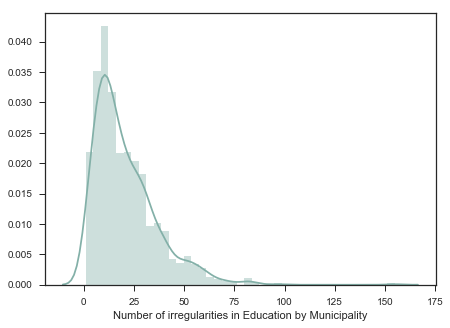
\includegraphics[width=1\textwidth]{n_irreg_EDUC.png}
     \end{center}
\end{column}
\begin{column}{0.5\textwidth}  %%<--- here
    \begin{center}
     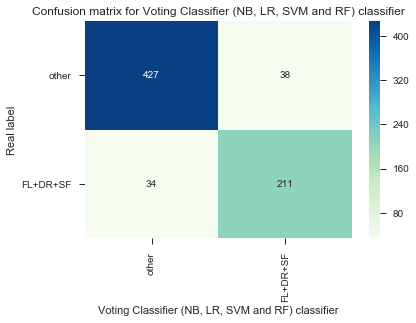
\includegraphics[width=1\textwidth]{matrix_mun.png}
     \end{center}
\end{column}
\end{columns}
\caption{\footnotesize{{\color{emap-azul-escuro}Figure:} Number of Irregularities in Education Frequency Distribution and Confusion matrix for the classification of municipalities}}
\end{itemize}
\centering

\end{frame}


%--------------------------------------------------------------------------------


\begin{frame}{Case Study: Does Corruption affect Educational Outcomes?}
\justifying
As an application of this framework we propose replicating the empirical strategy proposed by~ Ferraz, Finan and Moreira (2012)\nocite{Educacao}, that estimates the relationship between corruption in educational transfers and schooling outcomes:

\begin{align*}
    \label{eq:modelo}
        A_{s,m,4} &= \alpha + \beta C_m + Z'_m \theta_1 + X'_{s,m} \theta_2 + \epsilon_{s,m},
    \end{align*}
    
\begin{itemize}
\small
    \item [--] $A_{s,m,4}$ is a vector of average student achievements for each school \textit{s} in the 4th grade,
    \item [--] $C_m$ is a measure of corruption in education,
    \item [--] $Z_m$ is a vector of municipal characteristics,
    \item [--] $X_{s,m}$ is a vector of students characteristics, aggregated by school.
\end{itemize}
\end{frame}



\begin{frame}{Case Study}
\justifying
\small
Since we have irregularities detected in audits taken in three political terms (2005-2008, 2009-2012, 2013-2016), we gathered data for available years within this range.
\vspace{1em}

{\color{emap-azul-escuro}Educational outcomes and school characteristics:}
\begin{itemize}
\justifying
    \item [--] Math and Portuguese scores, selected Students and Principals surveys answers from Prova Brasil/SAEB, INEP.
    \item [--] Failure and Dropout rates, existence of computer lab, science lab and sanitation from School Census, INEP.
\end{itemize}
\vspace{1em}

{\color{emap-azul-escuro} Municipal characteristics:}
\begin{itemize}
\justifying
    \item [--] Gini and Population from 2010 Census, IBGE.
    \item [--] GDP per-capita from Gross Domestic Product of Municipalities, IBGE.
    \item [--] Municipal spending per pupil in primary education from SIOPE, MEC.
\end{itemize}
\end{frame}



\begin{frame}{Case Study}


\begin{figure}[h!]
%\label{fig:distClass}
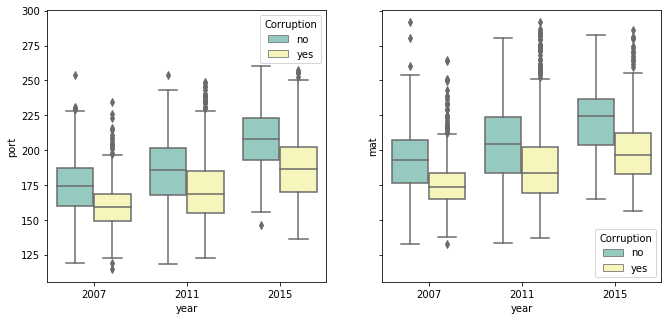
\includegraphics[width=9cm]{port_mat_grave.png}
\centering
\caption{Portuguese and Math ccores on Prova Brasil, split by term and incidence of corruption in Education}
\end{figure}
\small
\justifying
Note: Among 4,670 schools, approximately 49\% are in municipalities where exists corruption in Education, according to our indicator.
\end{frame}


\begin{frame}{Case Study}


\begin{figure}[h!]
%\label{fig:distClass}
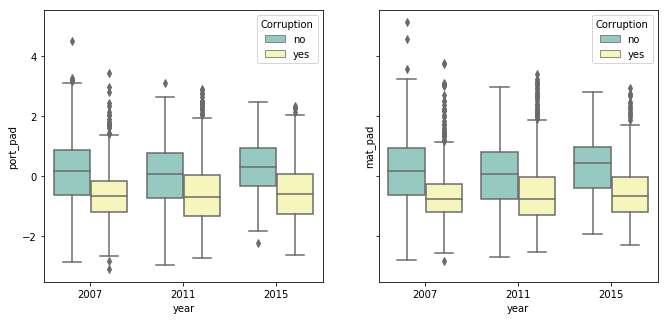
\includegraphics[width=9cm]{port_mat_pad_grave.png}
\centering
\caption{Portuguese and Math standardized scores on Prova Brasil, split by term and incidence of corruption in Education}
\end{figure}
\end{frame}


\begin{frame}{Case Study}
\justifying
\vspace{0.5em}
\small

\begin{table}[h!]
\centering
\caption{\small Parameters specification to adjust for Measurement error}
\label{fork}
\small
\begin{tabular}{p{4cm}C{4cm}C{4cm}}
\toprule
\textbf{Parameter} & \textbf{Negative Binomial}  & \textbf{Classification task} \\
{} & (1) &  (2)\\\midrule
$P$ & 0.35 &  0.35  \\
$r_0$ &  0.055 & 0.078\\
$r_1$   &  0.186 &  0.104\\\midrule
term inv-cov.  &  5.35 &  5.35\\\midrule
term of adjustment &  1.67 &  1.38\\
\bottomrule
\end{tabular}

\end{table}


\end{frame}


\begin{frame}{Case Study}
\justifying
\begin{table}[h!]
    \centering
    \caption{Effects of Corruption on Mathematics Standardized Test Scores}
    \label{math}
    \small
\begin{tabular}{p{3.5cm} m{2.7cm} *{2}{m{.1\linewidth}}}
\toprule
{} & \textbf{OLS Estimation} & \multicolumn{2}{l}{\textbf{MLS Estimation}} \\ 
{} & {} & (1) & (2)  \\\midrule
Corruption & -0.1098***  &  -0.183***   & -0.152*** \\
in Education &    (0.025)    &   (0.042)   &   (0.035)  \\
{} & {} & {} & {}\\\midrule
School and Municipal characteristics   & Yes & Yes & Yes\\
\bottomrule
\end{tabular}

\scriptsize{Dependent Variable: Standardized Math Test scores among 5th year students.  

Robust SE. Adjusted R-squared for OLS Estimation: 0.497. $N=4670$}
\end{table}
\end{frame}


\begin{frame}{Case Study}
\justifying
\begin{table}[h!]
    \centering
    \caption{Effects of Corruption on Portuguese Standardized Test Scores}
    \label{port}
    \small
\begin{tabular}{p{3.5cm} m{2.7cm} *{2}{m{.1\linewidth}}}
\toprule
{} & \textbf{OLS Estimation} & \multicolumn{2}{l}{\textbf{MLS Estimation}} \\ 
{} & {} & (1) & (2)  \\\midrule
Corruption & -0.111***  &  -0.185***   & -0.153*** \\
in Education &    (0.024)    &   (0.04)   &   (0.033)  \\
{} & {} & {} & {}\\\midrule
School and Municipal characteristics  & Yes & Yes & Yes\\
\bottomrule
\end{tabular}

\scriptsize{Dependent Variable: Standardized Portuguese Test scores among 5th year students.

Robust SE. Adjusted R-squared for OLS Estimation: 0.534. $N=4670$}
\end{table}
\end{frame}


\begin{frame}{Case Study}
\justifying
\begin{table}[h!]
    \centering
    \caption{Effects of Corruption on Dropout Rates}
    \label{drop}
    \small
\begin{tabular}{p{3.5cm} m{2.7cm} *{2}{m{.1\linewidth}}}
\toprule
{} & \textbf{OLS Estimation} & \multicolumn{2}{l}{\textbf{MLS Estimation}} \\ 
{} & {} & (1) & (2)  \\\midrule
Corruption & 0.003**  &  0.005***   &  0.004***\\
in Education &    (0.001)    &   (0.002)   &  (0.001)   \\
{} & {} & {} & {}\\
School and Municipal characteristics  & Yes & Yes & Yes\\
\bottomrule
\end{tabular}

\scriptsize{Dependent Variable: Dropout rates among 5th year students.

Robust SE. Adjusted R-squared for OLS Estimation: 0.209. $N=4670$}
\end{table}
\end{frame}



\begin{frame}{Case Study}
\justifying
\begin{table}[h!]
    \centering
    \caption{Effects of Corruption on Failure Rates}
    \label{fail}
    \small
\begin{tabular}{p{3.5cm} m{2.7cm} *{2}{m{.1\linewidth}}}
\toprule
 & \textbf{OLS Estimation} & \multicolumn{2}{l}{\textbf{MLS Estimation}} \\ 
 & {} & (1) & (2)  \\\midrule
Corruption & 0.006*  &  0.009**   &  0.008**\\
in Education &    (0.003)    &  (0.005)    & (0.004) \\
{} & {} & {} & {}\\\midrule
School and Municipal characteristics  & Yes & Yes & Yes\\
\bottomrule
\end{tabular}

\scriptsize{Dependent Variable: Failure rates among 5th year students.

Robust SE. Adjusted R-squared for OLS Estimation: 0.175. $N=4670$}
\end{table}
\end{frame}


\section{Conclusion}

\begin{frame}{Conclusion}
\justifying
\vspace{1em}
\small

In this study we proposed a framework to guide the efficient use of text data in inferential models, taking Audit reports from the CGU Anti-Corruption program as a particular application.

\vspace{1em}
Overall, we obtained satisfactory results using the proposed framework, both on the machine learning classification step and on the regression model estimation.

\vspace{1em}
Nevertheless, we understand that it has some limitations to be addressed in future works:
\begin{itemize}
\small
\justifying
    \item The framework was initially designed to construct and deal with measurement error in a binary indicator, but a natural extension is to adapt it for other variables, such as proportion and mean.
    \item Although we proposed a particular use case, we expect this framework to be useful with other sources of text data, accounting for differences in structure and vocabulary. 
\end{itemize} 

\vspace{1em}


\end{frame}

% -----------------------------------------------------------------------------


%\nocite{*}
\section{References}

\begin{frame}[allowframebreaks]{References}

\bibliographystyle{abbrvnat}
\bibliography{references}

\end{frame}

\end{document}